%; whizzy paragraph -pdf xpdf -latex ./whizzypdfptex.sh
%; whizzy-paragraph "^\\\\begin{frame}\\|\\\\emtext"
% latex beamer presentation.
% platex, latex-beamer $B$G%3%s%Q%$%k$9$k$3$H$rA[Dj!#(B

%     Tokyo Debian Meeting resources
%     Copyright (C) 2012 Junichi Uekawa
%     Copyright (C) 2016 Nobuhiro Iwamatsu

%     This program is free software; you can redistribute it and/or modify
%     it under the terms of the GNU General Public License as published by
%     the Free Software Foundation; either version 2 of the License, or
%     (at your option) any later version.

%     This program is distributed in the hope that it will be useful,
%     but WITHOUT ANY WARRANTY; without even the implied warreanty of
%     MERCHANTABILITY or FITNESS FOR A PARTICULAR PURPOSE.  See the
%     GNU General Public License for more details.

%     You should have received a copy of the GNU General Public License
%     along with this program; if not, write to the Free Software
%     Foundation, Inc., 51 Franklin St, Fifth Floor, Boston, MA  02110-1301 USA

\documentclass[cjk,dvipdfmx,12pt]{beamer}
\usetheme{Tokyo}
\usepackage{monthlypresentation}

%  preview (shell-command (concat "evince " (replace-regexp-in-string "tex$" "pdf"(buffer-file-name)) "&")) 
%  presentation (shell-command (concat "xpdf -fullscreen " (replace-regexp-in-string "tex$" "pdf"(buffer-file-name)) "&"))
%  presentation (shell-command (concat "evince " (replace-regexp-in-string "tex$" "pdf"(buffer-file-name)) "&"))

%http://www.naney.org/diki/dk/hyperref.html
%$BF|K\8l(BEUC$B7O4D6-$N;~(B
\AtBeginDvi{\special{pdf:tounicode EUC-UCS2}}
%$B%7%U%H(BJIS$B7O4D6-$N;~(B
%\AtBeginDvi{\special{pdf:tounicode 90ms-RKSJ-UCS2}}

\newenvironment{commandlinesmall}%
{\VerbatimEnvironment
  \begin{Sbox}\begin{minipage}{1.0\hsize}\begin{fontsize}{8}{8} \begin{BVerbatim}}%
{\end{BVerbatim}\end{fontsize}\end{minipage}\end{Sbox}
  \setlength{\fboxsep}{8pt}
% start on a new paragraph

\vspace{6pt}% skip before
\fcolorbox{dancerdarkblue}{dancerlightblue}{\TheSbox}

\vspace{6pt}% skip after
}
%end of commandlinesmall

\newcommand{\textframe}[1]{
	\begin{frame}{}
	\begin{center}
	 {\Huge #1
		  }
	 \end{center}
	 \end{frame}
}


\title{Raspberry Pi3 / arm64}
\subtitle{Debian/Ubuntu $B%_!<%H%"%C%W(B in $B;%KZ(B}
\author{$B4d>>(B $B?.MN(B}
\date{2016$BG/(B6$B7n(B17$BF|(B}
\logo{
\includegraphics[width=8cm]{image200607/openlogo-light.eps}}

\begin{document}

\begin{frame}
\titlepage{}
\end{frame}


\begin{frame}{$B<+8J>R2p(B}

\begin{itemize}
\item $BL>A0(B: $B4d>>(B $B?.MN!J$$$o$^$D(B $B$N$V$R$m!K(B @iwamatsu
\item Debian Project Official Developer
\item Debian $B$G$N$*;E;v(B: Debian linux kernel, Debian Bluetooth, Debian Science (OpenCV), Erlang, Debian Go
\item $BIaCJ$N$*;E;v(B: Linux kernel $B3+H/!"(BU-Boot $B%a%s%F%J!"(BYocto Project
\end{itemize} 
\end{frame}

%\begin{frame}{Agenda}
%  \begin{itemize}
%   \item Debian $B$H$O!)(B
%   \item Debian Updates
%   \item $B:#8e$N%$%Y%s%H(B
%  \end{itemize}
%\end{frame}
%
%\section{Debian $B$H$O!)(B}
%\begin{frame}\begin{center}\Huge{Debian $B$H$O!)(B}\end{center}\end{frame}

\begin{frame}{Raspberry Pi 3/RPi3}

\begin{itemize}
\item 2016/2/29 $BHNGd3+;O(B
\item Broadcom BCM2837 Cortex-A53 1.2Ghz Quad-core
\item aarch64 (ARM 64bit)
\item $B%a%b%j(B 1GB
\item WiFi$B$H(BBluetooth $BEk:\(B
\end{itemize}

\begin{center}
%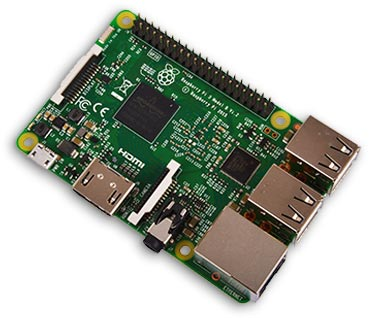
\includegraphics[width=0.5\hsize]{image201606/3141592653.jpg}
\end{center}
{\tiny \url{http://uk.rs-online.com/web/generalDisplay.html?id=raspberrypi}$B$h$j!#(B}

\end{frame}

\begin{frame}{Raspberry Pi 3/RPi3}

\begin{itemize}
\item $B%G%U%)%k%H(B $B%5%]!<%H(BOS
\begin{itemize}[<+->]
	\item Raspbian
	\item \color{red}{armhf ($BIbF0>.?tE@1i;;%O!<%I%&%'%"%5%]!<%H(B)}
	\item \color{red}{32bit$B%P%$%J%j!#(B64bit $B$G$O$J$$(B}
\end{itemize}
\end{itemize}

\end{frame}

\begin{frame}{Raspberry Pi 3/RPi3}

\begin{itemize}
\item $B%O!<%I%&%'%"$,(B64bit$B$J$N$K%=%U%H%&%'%"$O(B32bit$B$N$_%5%]!<%H(B
\item 64bit $B$N287C$r<u$1$?$$!#(B

\begin{itemize}
	\item $B9qFb$GMF0W$K9XF~$G$-$k5.=E$J(Baarch64$B%G%P%$%9(B
	\item $B%l%8%9%?%5%$%:!"%"%I%l%96u4V(B
	\item etc
\end{itemize}
\item $B%$%s%?!<%M%C%H>e$GM-;V$K$h$k0\?"$,3+;O$5$l$k!#(B
\end{itemize}

\end{frame}

\begin{frame}{RPi3 Linux arm64$B2=$^$G$NNr;K(B}

\begin{enumerate}[<+->]
\item RPi3 $BHNGdEv=i$O(B32bit $B$N$_BP1~(B \\
   stub ($B%G%P%$%9=i4|%W%m%0%i%`(B) $B$,(B 32bit $B%5%]!<%H$N$_!#(B\\
   Linux$B%+!<%M%k$bL$BP1~!#(B\\
   $BAaB.(BRpi $B$N%U%)!<%i%`$G(B64bit$B2=$NOCBj$,:n@.$5$l$k!#(B\\
   \ \ {\tiny \url{https://www.raspberrypi.org/forums/viewtopic.php?f=66&t=138385}}

\item 2016/3/26 $B$K(BGithub $B$K%P%0%l%]!<%H$5$l$k!#(B\\
   \ \ {\tiny \url{https://github.com/raspberrypi/firmware/issues/579}}
\end{enumerate}
\end{frame}

\begin{frame}{RPi3 Linux arm64$B2=$^$G$NNr;K(B}
\begin{enumerate}
\setcounter{enumi}{3}
\item Stephen Warren $B;a(B(U-Boot / Nvidia / Rpi $B%a%s%F%J(B) $B$K$h$C$F(B stub $B$,3+H/$5$l$k!#(B
   \ \ {\tiny \url{https://github.com/swarren/rpi-3-aarch64-demo}}

\item Raspberry Pi Foundation $B$,(B 64bit(armv8) $B8~$1(Bstub$B$r8x3+!#(B \\
   \ \ {\tiny \url{https://github.com/raspberrypi/tools.git}}

\end{enumerate}
\end{frame}

\textframe{RPi3 Linux arm64 $B%5%]!<%H>u67(B}

\begin{frame}[containsverbatim]{$B%/%m%9%3%s%Q%$%i(B}

Debian stretch/sid $B$G$O(B $B8x<0%j%]%8%H%j$+$i%$%s%9%H!<%k2DG=!#(BUbuntu$B$bF1MM$K2DG=!#(B

\begin{commandline}
$ sudo apt install gcc-aarch64-linux-gnu
\end{commandline}
%$

\end{frame}

\begin{frame}{$B%V!<%H%m!<%@(B}

\begin{itemize}
\item $B4pK\%V!<%H%m!<%@ITMW$J%G%P%$%9$@$,!"(BRPi3/aarch64 Linux$B%+!<%M%k$,3+H/ESCf$N$?$a(B
$B$$$m$$$m$$$8$l$k$h$&$K$9$k$?$a$K%M%C%H%o!<%/(B/USB$B%V!<%H$,$G$-$k$h$&4D6-$r@0$((B
$B$F$*$$$?$[$&$,3Z!#(B
\item $BAH9~5!4o$G$h$/MxMQ$5$l$k(BU-Boot$B$r$G$O4{$K%5%]!<%H$5$l$F$$$k$?$a!"(BSD$B%+!<%I$KAH$_9~$s$G(B
$BCV$/!#(B
	{\small \url{git://git.denx.de/u-boot.git}}
\end{itemize}

\begin{center}
\includegraphics[width=0.8\hsize]{image201606/boot.eps}
\end{center}

\end{frame}

\begin{frame}{Linux $B%+!<%M%k(B}

\begin{itemize}
  \item LKML$B$K$O%5%]!<%HMQ%Q%C%A$,Ej9F$5$l$F$$$k!#(B4.8$B!"(B4.9 $B$K$O%5%]!<%H$,F~$kF0$-!#(B
  \begin{center}
  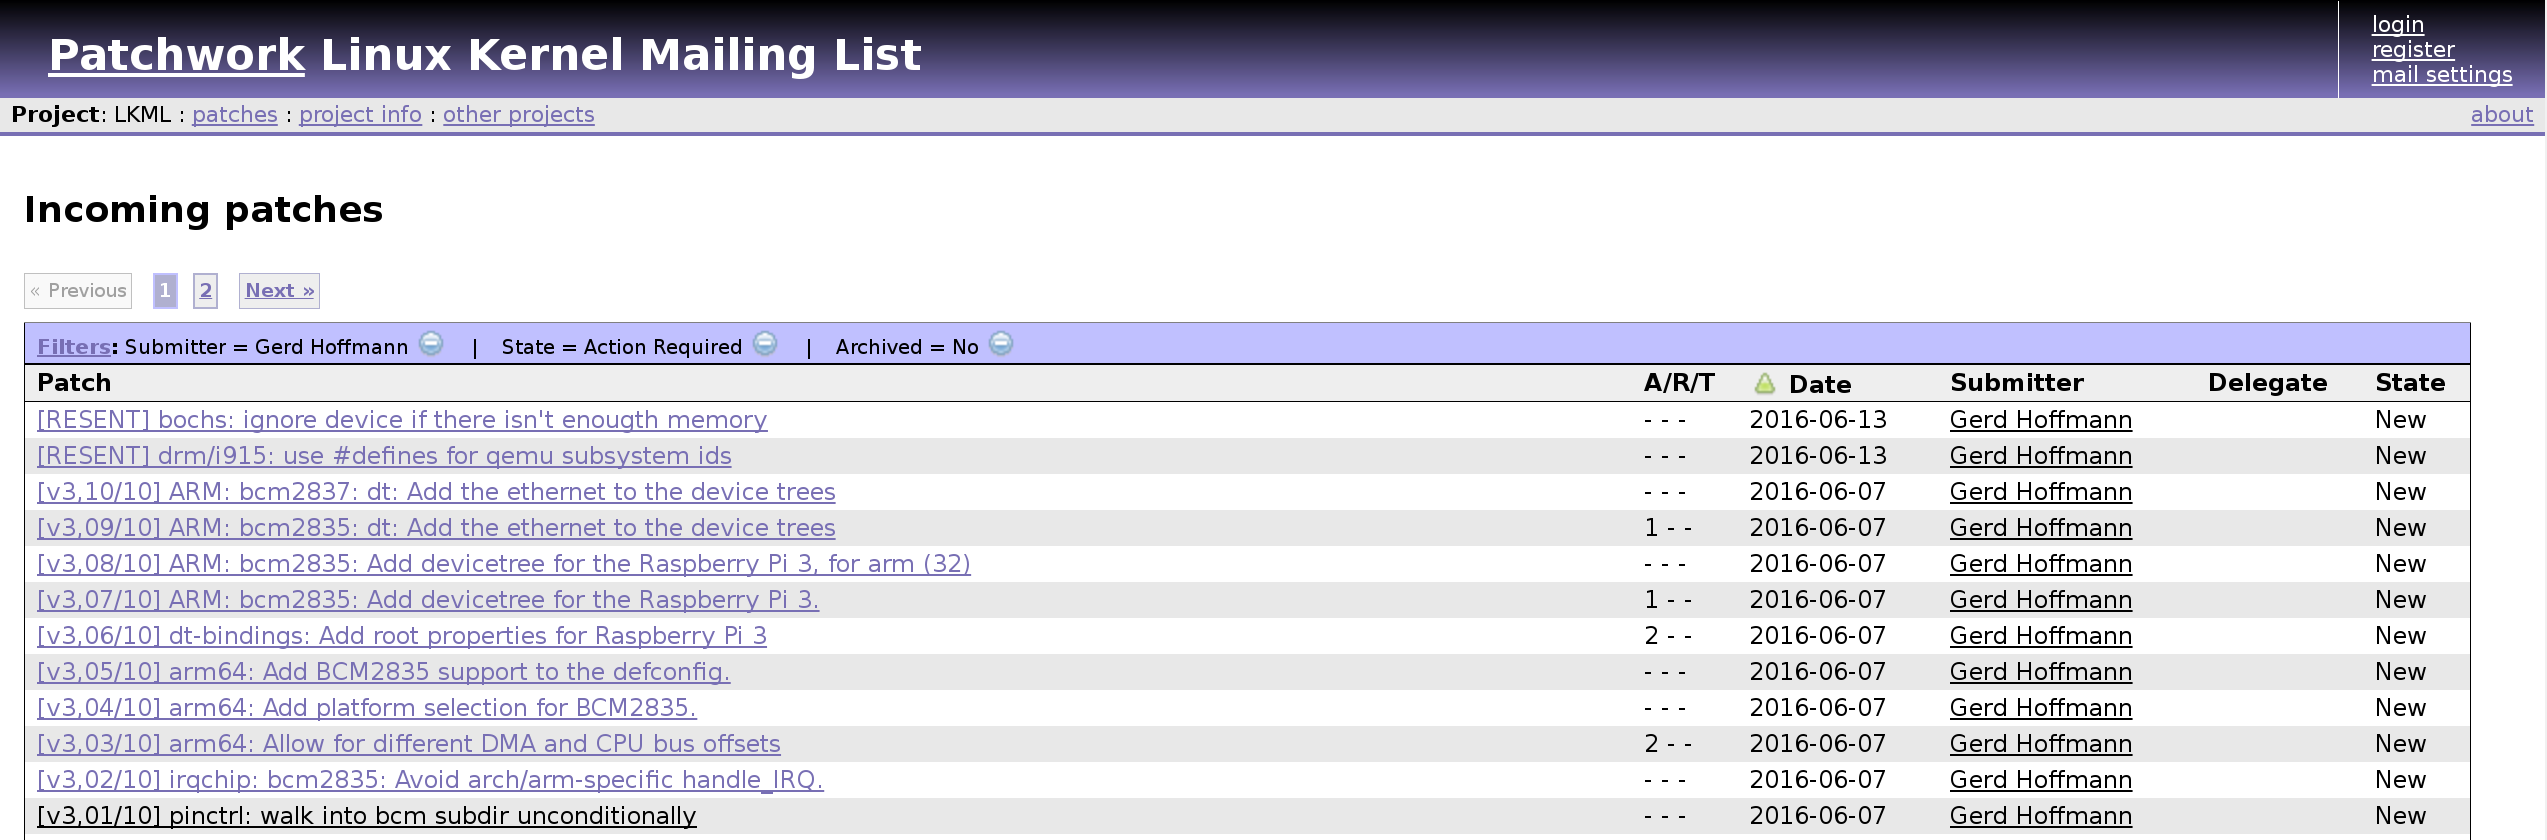
\includegraphics[width=0.8\hsize]{image201606/patchwork.png}
  \end{center}
  \item Raspberry Pi Foundation $B$G$O$^$@L$%5%]!<%H!#(B \\
   \ \ {\small \url{https://github.com/raspberrypi/linux/issues/1310}}
  \item $BM-;V$K$h$C$F8x3+$5$l$F$$$k(BLinux$B%+!<%M%k$,$$$/$D$+B8:_!#(B\\
    \ \ {\small \url{https://github.com/anholt/linux.git}} \\
    \ \ {\small \url{https://github.com/zeldin/linux.git}} \\
\end{itemize}

\end{frame}

\begin{frame}{$B%f!<%6%i%s%I(B}

\begin{itemize}
  \item Debian / Ubuntu $B$G(B aarch64$B8~$1%P%$%J%j$,Ds6!!#(B
  \item RedHat, Suse$B!"(BGentoo$B!"(BArch$B$J$I$N<gMW%G%#%9%H%j$G$b%5%]!<%H!#(B
\end{itemize}

\end{frame}

\textframe{RPi3 Debian/arm64 $B2=J}K!(B}

\begin{frame}{arm64$B2=$NN.$l(B}

\begin{enumerate}
  \item $B%/%m%9%3%s%Q%$%i$N%$%s%9%H!<%k(B
  \item microSD$B%+!<%I$N%U%)!<%^%C%H!&%Q!<%F%#%7%g%s:n@.(B
  \item RPi3 $B%V!<%H%U%!%$%k$N<hF@$H(B/boot$B$X$N%3%T!<(B
  \item U-Boot$B$N%=!<%9%3!<%I<hF@$H%3%s%Q%$%k(B
  \item Linux $B%+!<%M%k%=!<%9%3!<%I$N%3%s%Q%$%k(B
  \item cdebootstrap $B$r;H$C$?(BmicroSD$B%+!<%I$X$N%f!<%6%i%s%I%$%s%9%H!<%k(B
\end{enumerate}

\end{frame}

\textframe{1. $B%/%m%9%3%s%Q%$%i$N%$%s%9%H!<%k(B}

\begin{frame}[containsverbatim]{$B%/%m%9%3%s%Q%$%i$N%$%s%9%H!<%k(B}
  \begin{commandline}
  $ sudo apt update
  $ sudo apt install gcc-aarch64-linux-gnu
  \end{commandline}
\end{frame}

\textframe{2. microSD$B%+!<%I$N%U%)!<%^%C%H!&%Q!<%F%#%7%g%s:n@.(B}

\begin{frame}[containsverbatim]{microSD$B%+!<%I$NG'<13NG'(B}

\begin{commandline}
$ dmesg  | tail -5
[869873.800361] sd 6:0:0:3: [sde] 15523840 512-byte logical blocks: (7.94 GB/7.40 GiB)
[869873.831121]  sde: sde1
\end{commandline}

\end{frame}

\begin{frame}[containsverbatim]{$B%Q!<%F%#%7%g%s%F!<%V%kNN0h$r=i4|2=(B}

\begin{commandline}
$ sudo dd if=/dev/zero of=/dev/sde bs=1M count=1
\end{commandline}
%$

\end{frame}

\begin{frame}[containsverbatim]{microSD$B%+!<%I$K%Q!<%F%#%7%g%s:n@.(B/1}

$BBh(B1$B%Q!<%F%#%7%g%s$O(B 32MB/FVAT $B%U%!%$%k%7%9%F%`!"(B
$BBh(B2$B%Q!<%F%#%7%g%s$O;D$j%5%$%:(B/EXT4 $B%U%!%$%k%7%9%F%`$H$7$F:n@.!#(B

\begin{commandline}
$ sudo fdisk /dev/sde
Command (m for help): o
...
Command (m for help): n
...
Select (default p): p
...
Partition number (1-4, default 1): 1
...
Last sector, +sectors or +size{K,M,G,T,P} \
	     (2048-15523839, default 15523839): +32M
...
\end{commandline}
%$

\end{frame}

\begin{frame}[containsverbatim]{microSD$B%+!<%I$K%Q!<%F%#%7%g%s:n@.(B/2}

\begin{commandline}
Command (m for help): t
...
Hex code (type L to list all codes): e
...
Command (m for help): n
...
Select (default p): p
...
Partition number (2-4, default 2): 2
...
Command (m for help): w
\end{commandline}

\end{frame}

\begin{frame}[containsverbatim]{microSD$B%+!<%I$K%Q!<%F%#%7%g%s:n@.(B $B%o%s%i%$%J!<HG(B}
\begin{commandline}
(echo o; echo n; echo p; echo 1; echo ; echo +32M; \
 echo t; echo e; echo n; echo p; echo 2; echo ; echo ; \
 echo w) | fdisk /dev/sde
\end{commandline}
\end{frame}

\begin{frame}[containsverbatim]{microSD$B%+!<%I$N%U%)!<%^%C%H(B}
\begin{commandline}
$ sudo mkfs.msdos /dev/sde1
$ sudo mkfs.ext4 /dev/sde2
$ mkdir /tmp/boot /tmp/rootfs
$ sudo mount /dev/sde1 /tmp/boot
$ sudo mount /dev/sde2 /tmp/rootfs
\end{commandline}
\end{frame}

\textframe{3. RPi3 $B%V!<%H%U%!%$%k$N<hF@$H(B/boot$B$X$N%3%T!<(B}

\begin{frame}[containsverbatim]{RPi3 $B%V!<%H%U%!%$%k$N<hF@$H(B/boot$B$X$N%3%T!<(B}

  \begin{commandline}
  $ git clone --depth 1 \ 
  	https://github.com/raspberrypi/tools.git
  $ sudo cp -rf tools/boot/* /tmp/boot/
  \end{commandline}
\end{frame}

\textframe{4. U-Boot$B$N%=!<%9%3!<%I<hF@$H%3%s%Q%$%k(B}

\begin{frame}[containsverbatim]{U-Boot$B$N%=!<%9%3!<%I<hF@$H%3%s%Q%$%k(B}
  \begin{commandline}
  $ git clone git://git.denx.de/u-boot.git
  $ cd u-boot
  $ make rpi_3_defconfig
  $ make CROSS_COMPILE=aarch64-linux-gnu-
  $ sudo cp u-boot.bin /tmp/boot/
  $ cd ..
  \end{commandline}
\end{frame}

\begin{frame}[containsverbatim]{U-Boot$BMQ%9%/%j%W%H$N:n@.$H%3%T!<(B}
\begin{commandline}
$ cat << EOF > boot.scr
fatload mmc 0:1 \${fdt_addr_r} \${fdtfile}
fatload mmc 0:1 \${kernel_addr_r} image
setenv bootargs console=ttyS0,115200 \
	root=/dev/mmcblk0p2 rootfstype=ext4 rootwait rw
booti \${kernel_addr_r} - \${fdt_addr_r}
EOF
$ mkimage -A arm -O linux -T script -C none -a 0 \
	-e 0 -n "For Rpi3" -d boot.scr boot.scr.uimg
$ sudo cp boot.scr.uimg /tmp/boot/
\end{commandline}
\end{frame}

\begin{frame}[containsverbatim]{RPi3 $B%V!<%HJ}K!@_Dj(B(config.txt)}
\begin{commandline}
$ cat << EOF | sudo tee /tmp/boot/config.txt > /dev/null
enable_uart=1
arm_control=0x200
kernel=u-boot.bin
hdmi_group=2
hdmi_mode=82
EOF
\end{commandline}
\end{frame}

\textframe{5. Linux $B%+!<%M%k$N%=!<%9%3!<%I<hF@$H%3%s%Q%$%k(B}

\begin{frame}[containsverbatim]{Linux $B%+!<%M%k$N%=!<%9%3!<%I<hF@$H%3%s%Q%$%k(B}
\begin{commandline}
$ git clone https://github.com/anholt/linux.git
$ cd linux
$ git checkout -b rpi3-devel origin/bcm2837-64-next
$ make ARCH=arm64 CROSS_COMPILE=aarch64-linux-gnu-
$ sudo cp arch/arm64/boot/Image /tmp/boot/
$ sudo cp arch/arm64/boot/dts/broadcom/bcm2837-rpi-3-b.dtb \
	/tmp/boot/
\end{commandline}
\end{frame}

\textframe{6. cdebootstrap $B$r;H$C$?(BmicroSD$B%+!<%I$X$N%$%s%9%H!<%k(B}
\begin{frame}[containsverbatim]{cdebootstrap $B$r;H$C$?(BmicroSD$B%+!<%I$X$N%$%s%9%H!<%k(B}

\begin{commandline}
$ sudo cdebootstrap --arch=arm64 -f standard \
  --foreign jessie \
  --include=openssh-server,ntp,ca-certificates,vim \
  /tmp/rootfs
...
\end{commandline}

\end{frame}

\begin{frame}[containsverbatim]{fstab$B$N@_Dj(B}

\begin{commandline}
$ cat << EOF | \
	sudo tee /tmp/rootfs/etc/fstab > /dev/null
proc            /proc  proc defaults	     0 0
/dev/mmcblk0p1  /boot  vfat defaults	     0 2
/dev/mmcblk0p2  /      ext4 defaults,noatime 0 1
EOF
\end{commandline}
%$

\end{frame}

\begin{frame}[containsverbatim]{$B%M%C%H%o!<%/%G%P%$%9$N@_Dj(B}

\begin{commandline}
$ cat << EOF | \
	sudo tee /tmp/rootfs/etc/network/interfaces > \
	/dev/null
auto eth0
iface eth0 inet dhcp
\end{commandline}
%$

\end{frame}

\begin{frame}[containsverbatim]{rootfs$BMQ%Q!<%F%#%7%g%s$NJQ99(B}

\texttt{/tmp/rootfs/sbin/init} $B$rJT=8!#(B
\begin{commandline}
trap 'error "Interruped!"' HUP INT TERM

mount -n -o remount,rw rootfs / <- $B$3$l$r(B
mount -n -o remount,rw /dev/mmcblk0p2 / <- $B$3$l$KJQ99(B

chown -hR 0:0 /
\end{commandline}
\end{frame}

\begin{frame}[containsverbatim]{root $B$N%Q%9%o!<%I$N@_Dj$H(Brpi$B%f!<%6$NDI2C(B}
\begin{commandline}
echo 'deb http://ftp.debian.org/debian jessie main' > \
	     /etc/apt/sources.list

echo "root:root" | chpasswd <- $B$3$N9T$rDI2C(B
useradd -m rpi <- $B$3$N9T$rDI2C(B
echo rpi:rpi | chpasswd <- $B$3$N9T$rDI2C(B

run rm /sbin/init
\end{commandline}
\end{frame}

\begin{frame}[containsverbatim]{microSD$B%+!<%I$N%"%s%^%&%s%H$H(BRPi2$B$N5/F0(B}

\begin{enumerate}
\item microSD$B%+!<%I$r%"%s%^%&%s%H$7!"(BPpi3 $B$N(B microSD$B%+!<%I%9%m%C%H$KA^F~$9$k!#(B
\item $BA^F~8e!"(Bmicro USB $B%1!<%V%k$r(B Rpi3 $B$KA^$7!"(BRpi3$B$r5/F0$9$k!#(B
\item $B5/F0$9$k$H<+F0E*$K(B2nd bootstrap$B$,<B9T$5$l!"(BRpi3$B>e$G%$%s%9%H!<%k$,<B9T$5$l$k(B
\item 30$BJ,$[$IBT$D(B
\item $B%$%s%9%H!<%k40N;(B
\end{enumerate}
microSD$B%+!<%I$X$N>\:Y%$%s%9%H!<%kJ}K!$O(B 2015$BG/(B3$B7n$NJY6/2q;qNA(B
$B!V(BRapberry Pi 2 Model B $B$K(B Debian Jessie / armhf $B$r%$%s%9%H!<%k$9$k!W(B
$B$r;29M!#(B
\end{frame}

\textframe{$B%Y%s%A%^!<%/(B}
\begin{frame}[containsverbatim]{$B%Y%s%A%^!<%/(B}
Himeno Bench $B$GB,Dj(B
\begin{itemize}
	\item armhf (32bit)
		\begin{itemize}
			\item 1$B%3%";~(B: 79 MFLOPS
			\item 4$B%3%";~(B: 312 MFLOPS
		\end{itemize}
	\item aarch64 (64bit)
		\begin{itemize}
			\item 1$B%3%";~(B: 88 MFLOPS
			\item 4$B%3%";~(B: 334 MFLOPS
		\end{itemize}
\end{itemize}

1$B3d$[$IB.$$!#(B

\end{frame}
%
\textframe{$B$^$H$a(B}
\begin{frame}[containsverbatim]{$B$^$H$a(B}

\begin{itemize}
\item Rapberry Pi $BK\2H$G$O$^$@(Barm64$B$OL$%5%]!<%H$@$,!"M-;V$K$h$C$F4D6-$,@0$C$F$$$k!#(B
\item Linux Vanilla $B%+!<%M%k$NJ}$K%Q%C%A$,Ej9F$5$l$F$$$k!#(BLinux$B$G$N@5<0%5%]!<%H$b;~4V$N(B
$BLdBj$H;W$o$l$k!#(B
\item Himeno Bench$B$N7k2L$r8+$k8B$j!"(Barmhf $B$h$j(B1$B3d$[$IB.$$!#(B
\item $B%0%i%U%#%C%/$J$I$NBP1~$O$^$@L$D4::!#(B
\item arm64$B4D6-$G%+!<%M%k$J$I$NDc%l%$%d!<$G$$$m$$$mM7$S$?$$?M$K$O0\9T$9$k$h$$%?%$%_%s%0!#(B
\end{itemize}
\end{frame}

\end{document}

;;; Local Variables: ***
;;; outline-regexp: "\\([ 	]*\\\\\\(documentstyle\\|documentclass\\|emtext\\|section\\|begin{frame}\\)\\*?[ 	]*[[{]\\|[]+\\)" ***
;;; End: ***
